\subsection{Classification}
Our best training on the aforementioned dataset was made with 300 000 iterations over minibatches of size 32, with a learning rate decresaing 10 times throughout training. The full training took 5 days to finish on a Tesla K20C machine, and attained 70\% accuracy on network predictions, on a top-1 classification basis. Such results are satisfactory considering the resemblance of natural scene images. It should be noted that classification was not the main goal, but a good classification will intuitively lead to better class representations.

We can thus extract the trained filters responses to see images as processed by the network. The conv1 layer will mostly learn edges, namely the skyline and the waterline. Conv2 detects foliage, and convolutional layers 3 through 5 contain low-level features that are harder to interpret properly. We tested prototype generation on all convolutional layers, as well as the last pooling layer pool5, shown in fig.~\ref{prototypes}.

\begin{figure}[htb]
\centering
\begin{tabular}{cc}
    \bmvaHangBox{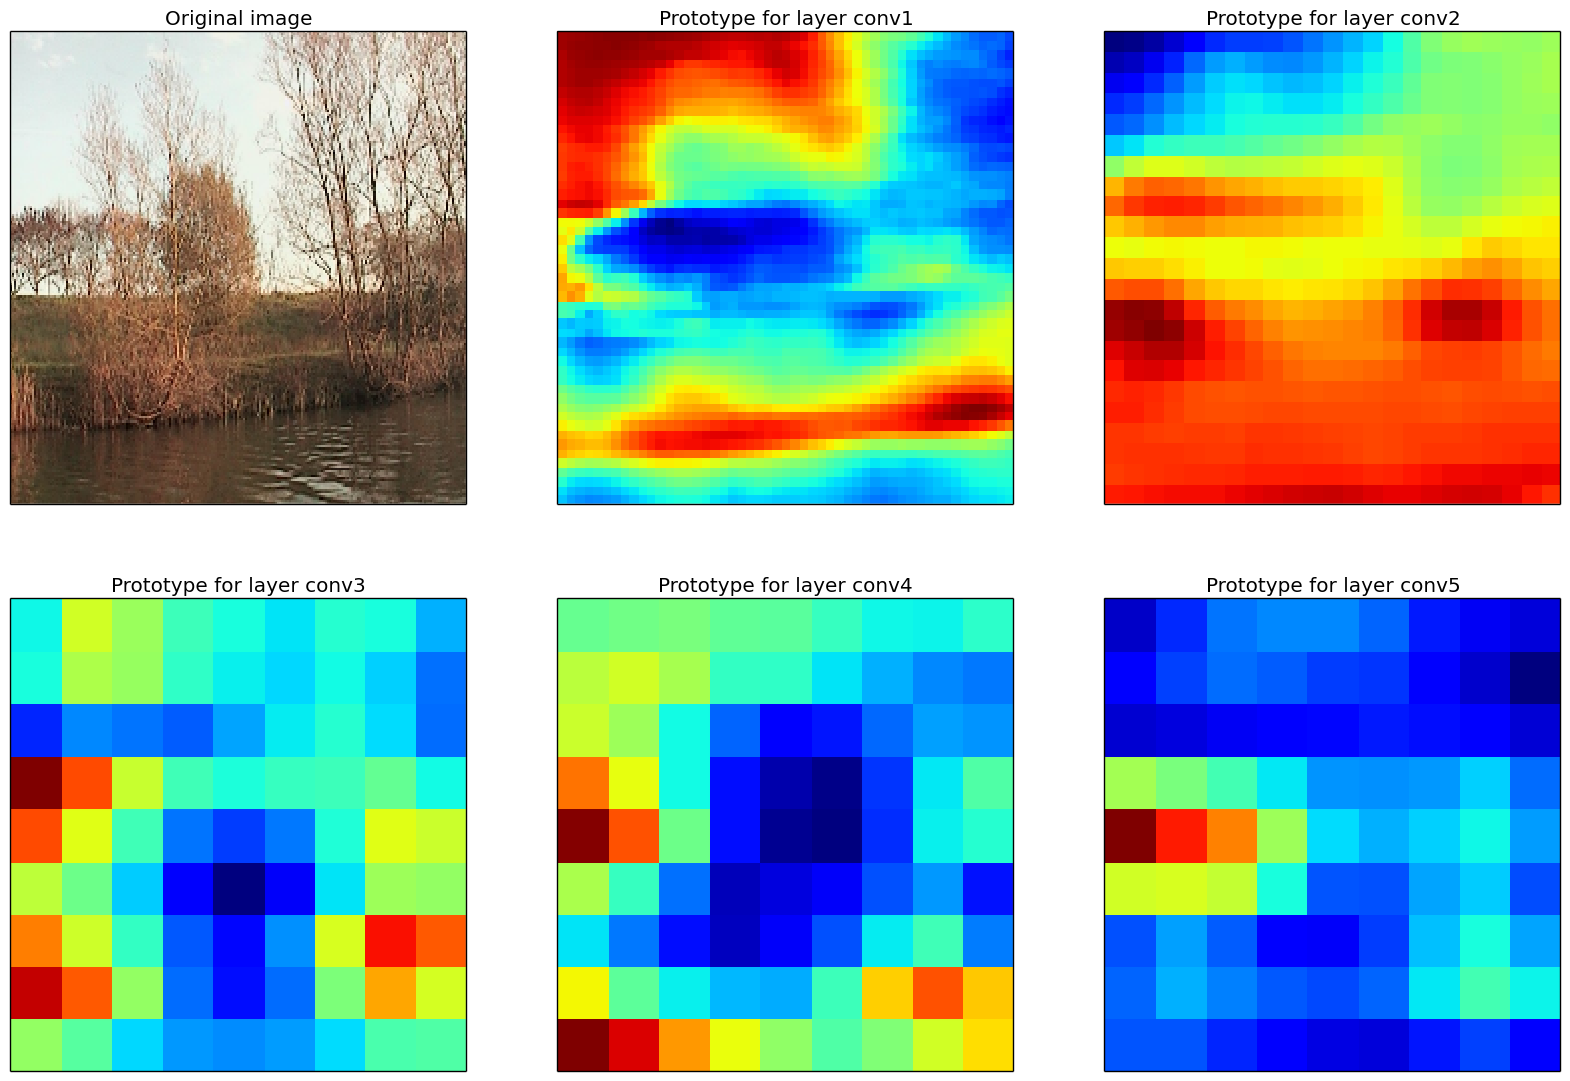
\includegraphics[width=0.9\linewidth]{images/classification/prototypes/avmaskplot7}}\\
\end{tabular}
\caption{Example of prototypes for a given image}
\label{prototypes}
\end{figure}

We generated prototypes for all classes, and tested whether an image can be recognized only using its class prototypes. Testing over a thousand random images and measuring using a cosine distance shows that all layers perform well for classification, with distances to the wrong prototype being indubitably larger than distances to the right prototype (fig.~\ref{fulltrainvalues} and \ref{allclft})

\begin{figure}[htb]
\centering
\begin{tabular}{|c|c|}
  \hline
   Layer & Ratio \\
  \hline
  conv1 & 1,766538663 \\
  conv2 & 2,994092459 \\
  conv3 & 1,866754565 \\
  conv4 & 1,796977461 \\
  conv5 & 1,681968205 \\
  pool5 & 1,860143028 \\
  \hline
\end{tabular}
\caption{Ratio of median distance for the wrong prototype over median distance for the right prototype}
\label{fulltrainvalues}
\end{figure}

\begin{figure}[htb]
\centering
\begin{tabular}{ccc}
    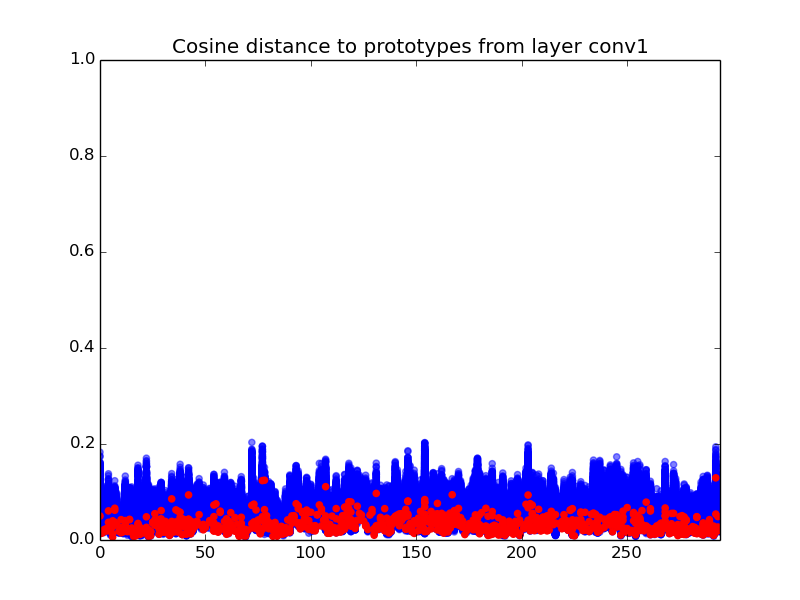
\includegraphics[width=0.33\linewidth]{images/classification/distances/all_classes_full_train/cos_distances_conv1}&
    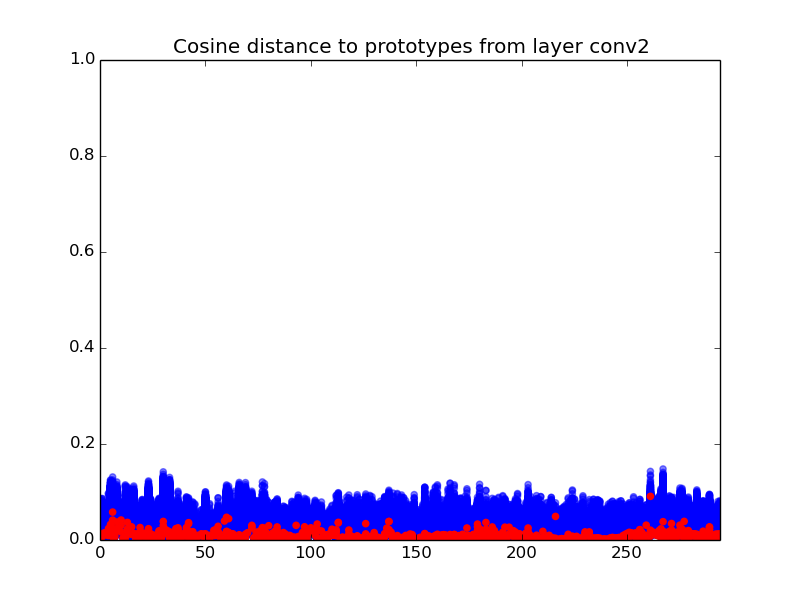
\includegraphics[width=0.33\linewidth]{images/classification/distances/all_classes_full_train/cos_distances_conv2}&
    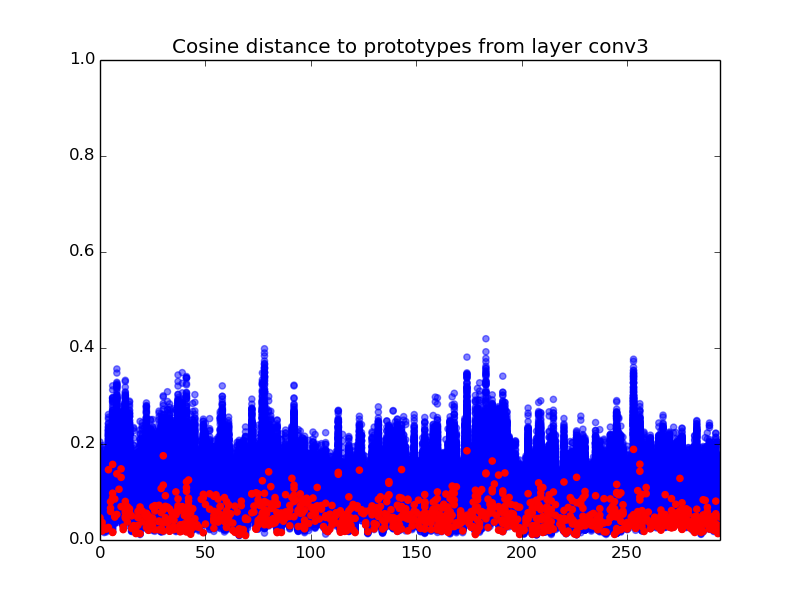
\includegraphics[width=0.33\linewidth]{images/classification/distances/all_classes_full_train/cos_distances_conv3} \\
    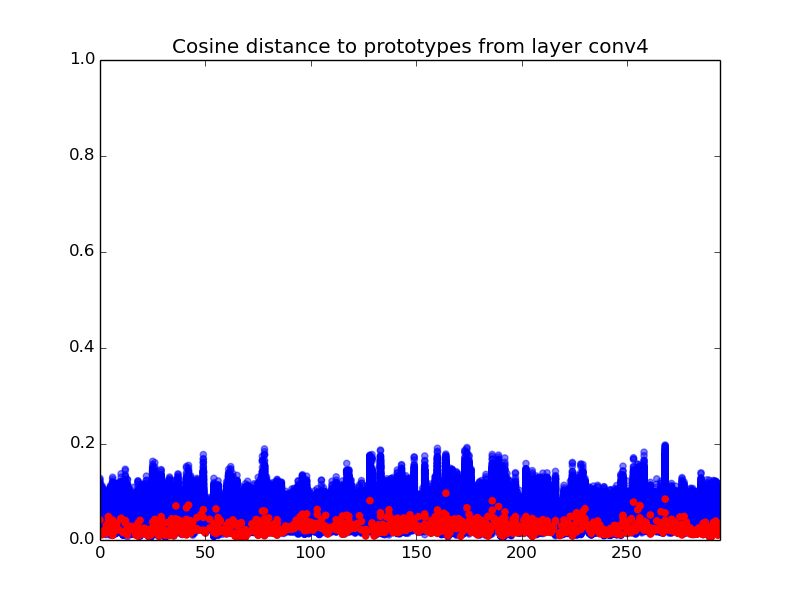
\includegraphics[width=0.33\linewidth]{images/classification/distances/all_classes_full_train/cos_distances_conv4}&
    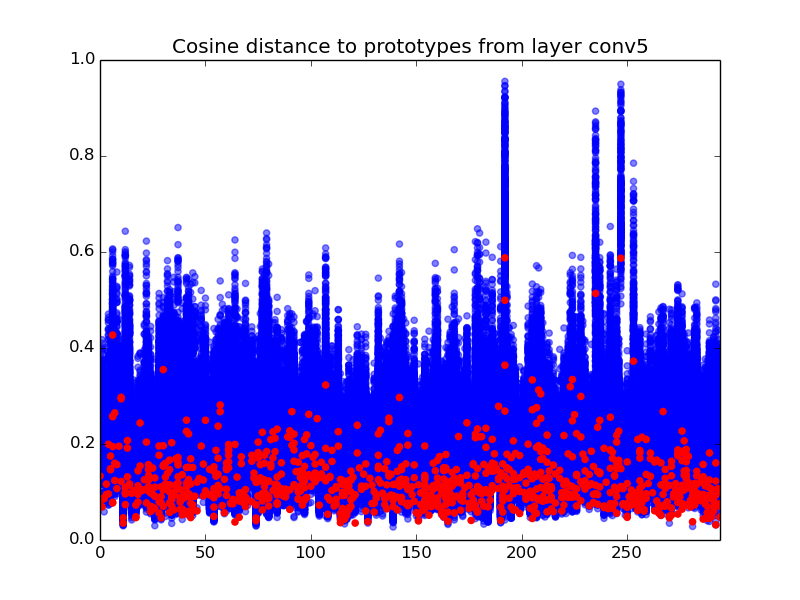
\includegraphics[width=0.33\linewidth]{images/classification/distances/all_classes_full_train/cos_distances_conv5}&
    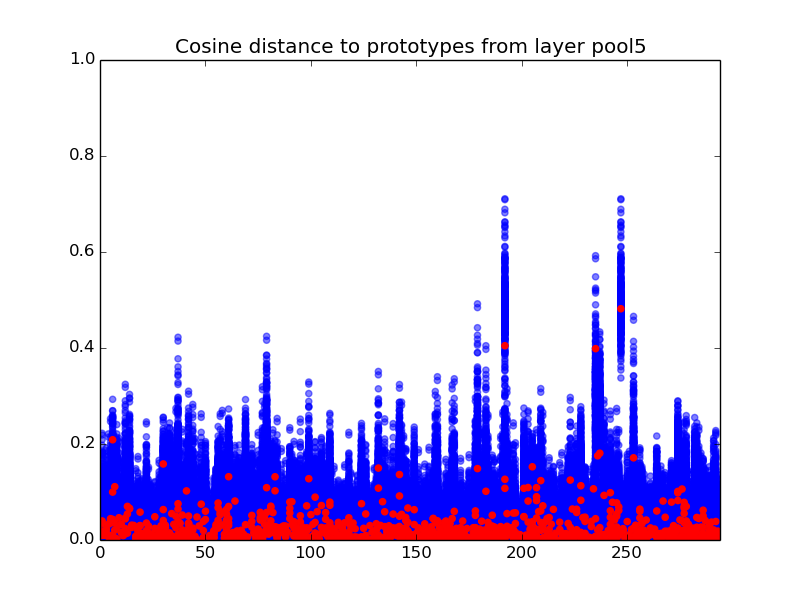
\includegraphics[width=0.33\linewidth]{images/classification/distances/all_classes_full_train/cos_distances_pool5} \\
\end{tabular}
\caption{Red dots represent the distance from a random class image to its class prototype, blue dots are distances to other class prototypes. Graphs show layers conv1 through pool5.}
\label{allclft}
\end{figure}

We also trained the same network on half the classes, to test for generalization capabilities. The results are analogous regarding known classes, but the network struggled with unseen classes (fig.~\ref{halftrainvalues}). It seems that it learns how to efficiently discriminate between its known classes, rather than truly recognizing a location.

\begin{figure}[htb]
\centering
\begin{tabular}{|c|c|c|}
  \hline
   Layer & Ratio (seen) & Ratio (unseen) \\
  \hline
  conv1 & 1,701451548 & 1,038455885 \\
  conv2 & 0,933561816 & 0,96491628 \\
  conv3 & 1,402536829 & 0,949963419 \\
  conv4 & 1,162658456 & 1,004402971 \\
  conv5 & 1,327277828 & 0,980390038 \\
  pool5 & 1,42521592 & 0,951486052 \\
  \hline
\end{tabular}
\caption{Ratio of median distances, for seen and unseen classes}
\label{halftrainvalues}
\end{figure}